\documentclass[border=0.125cm]{standalone}
\usepackage{tikz}
\usetikzlibrary{positioning}
\begin{document}

\tikzset{%
  every neuron/.style={
    circle,
    draw,
    minimum size=1cm
  },
  neuron missing/.style={
    draw=none, 
    scale=4,
    text height=0.333cm,
    execute at begin node=\color{black}$\vdots$
  },
}

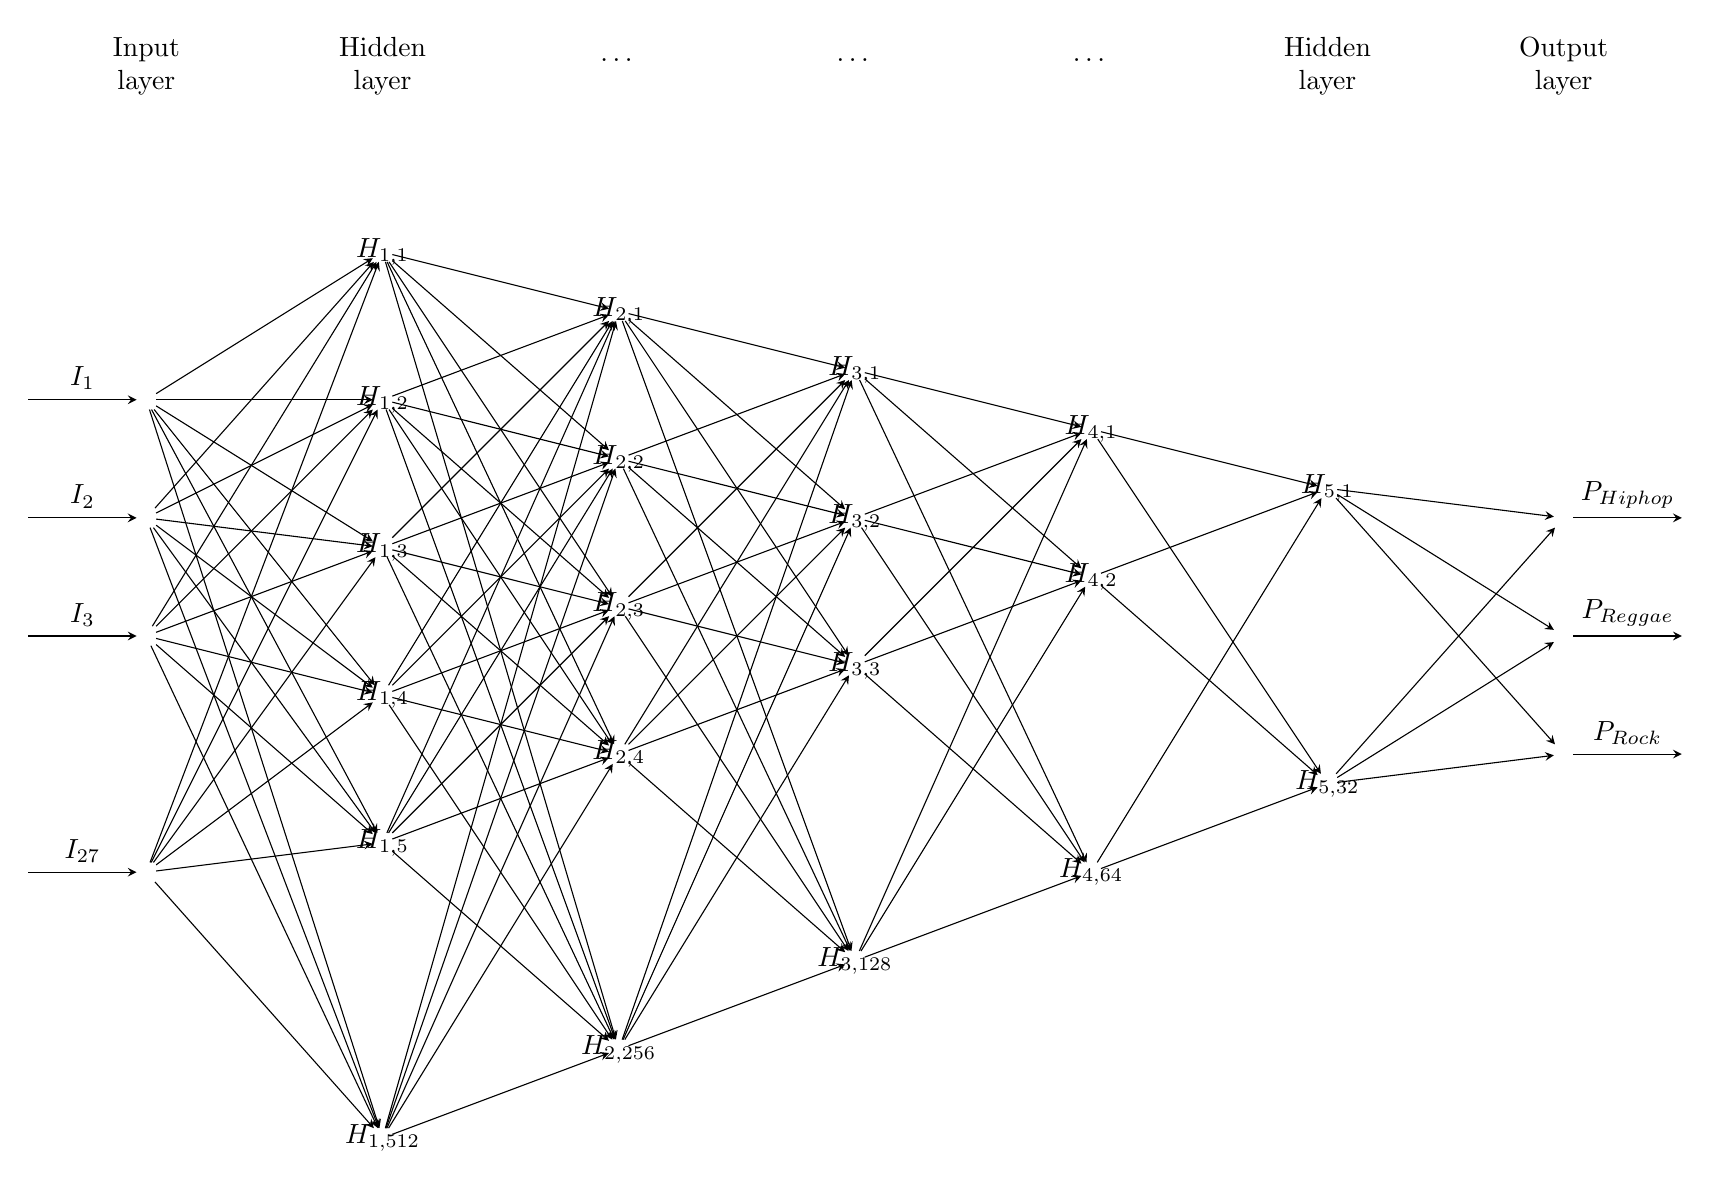
\begin{tikzpicture}[x=1.5cm, y=1.5cm, >=stealth]

\foreach \m/\l [count=\y] in {1,2,3,missing,4}
  \node [every neuron/.try, neuron \m/.try] (input-\m) at (0,.5-\y) {};

\foreach \m [count=\y] in {1,2,3,4,5,missing,6}
  \node [every neuron/.try, neuron \m/.try ] (hidden1-\m) at (2,2-\y*1.25) {};

\foreach \m [count=\y] in {1,2,3,4,missing,5}
\node [every neuron/.try, neuron \m/.try ] (hidden2-\m) at (4,1.5-\y*1.25) {};

\foreach \m [count=\y] in {1,2,3,missing,4}
\node [every neuron/.try, neuron \m/.try ] (hidden3-\m) at (6,1-\y*1.25) {};

\foreach \m [count=\y] in {1,2,missing,3}
\node [every neuron/.try, neuron \m/.try ] (hidden4-\m) at (8,0.5-\y*1.25) {};

\foreach \m [count=\y] in {1,missing,2}
\node [every neuron/.try, neuron \m/.try ] (hidden5-\m) at (10,-\y*1.25) {};

\foreach \m [count=\y] in {1,2,3}
  \node [every neuron/.try, neuron \m/.try ] (output-\m) at (12,-0.5-\y) {};

\foreach \l [count=\i] in {1,2,3,27}
  \draw [<-] (input-\i) -- ++(-1,0)
    node [above, midway] {$I_{\l}$};

\foreach \l [count=\i] in {1,2,3,4,5,512}
  \node [] at (hidden1-\i.center) {$H_{1,\l}$};

\foreach \l [count=\i] in {1,2,3,4,256}
	\node [] at (hidden2-\i.center) {$H_{2,\l}$};

\foreach \l [count=\i] in {1,2,3,128}
	\node [] at (hidden3-\i.center) {$H_{3,\l}$};

\foreach \l [count=\i] in {1,2,64}
\node [] at (hidden4-\i.center) {$H_{4,\l}$};

\foreach \l [count=\i] in {1,32}
\node [] at (hidden5-\i.center) {$H_{5,\l}$};


%\foreach \l [count=\i] in {1,2,3}
  \draw [->] (output-1) -- ++(1,0)
    node [above, midway] {$P_{Hiphop}$};
      \draw [->] (output-2) -- ++(1,0)
    node [above, midway] {$P_{Reggae}$};
      \draw [->] (output-3) -- ++(1,0)
    node [above, midway] {$P_{Rock}$};

\foreach \i in {1,...,4}
  \foreach \j in {1,...,6}
    \draw [->] (input-\i) -- (hidden1-\j);

\foreach \i in {1,...,6}
	\foreach \j in {1,...,5}
	\draw [->] (hidden1-\i) -- (hidden2-\j);

\foreach \i in {1,...,5}
	\foreach \j in {1,...,4}
	\draw [->] (hidden2-\i) -- (hidden3-\j);

\foreach \i in {1,...,4}
	\foreach \j in {1,...,3}
	\draw [->] (hidden3-\i) -- (hidden4-\j);

\foreach \i in {1,...,3}
	\foreach \j in {1,...,2}
	\draw [->] (hidden4-\i) -- (hidden5-\j);

\foreach \i in {1,...,2}
  \foreach \j in {1,...,3}
    \draw [->] (hidden5-\i) -- (output-\j);

\foreach \l [count=\x from 0] in {Input, Hidden}
  \node [align=center, above] at (\x*2,2) {\l \\ layer};

\foreach \l [count=\x from 0] in {\dots, \dots,\dots}
\node [align=center, above] at (4+\x*2,2) {\l \\};

\foreach \l [count=\x from 0] in {Hidden, Output}
\node [align=center, above] at (10+\x*2,2) {\l \\ layer};

\end{tikzpicture}

\end{document}